\documentclass[twoside]{book}

% Packages required by doxygen
\usepackage{fixltx2e}
\usepackage{calc}
\usepackage{doxygen}
\usepackage[export]{adjustbox} % also loads graphicx
\usepackage{graphicx}
\usepackage[utf8]{inputenc}
\usepackage{makeidx}
\usepackage{multicol}
\usepackage{multirow}
\PassOptionsToPackage{warn}{textcomp}
\usepackage{textcomp}
\usepackage[nointegrals]{wasysym}
\usepackage[table]{xcolor}

% Font selection
\usepackage[T1]{fontenc}
\usepackage[scaled=.90]{helvet}
\usepackage{courier}
\usepackage{amssymb}
\usepackage{sectsty}
\renewcommand{\familydefault}{\sfdefault}
\allsectionsfont{%
  \fontseries{bc}\selectfont%
  \color{darkgray}%
}
\renewcommand{\DoxyLabelFont}{%
  \fontseries{bc}\selectfont%
  \color{darkgray}%
}
\newcommand{\+}{\discretionary{\mbox{\scriptsize$\hookleftarrow$}}{}{}}

% Page & text layout
\usepackage{geometry}
\geometry{%
  a4paper,%
  top=2.5cm,%
  bottom=2.5cm,%
  left=2.5cm,%
  right=2.5cm%
}
\tolerance=750
\hfuzz=15pt
\hbadness=750
\setlength{\emergencystretch}{15pt}
\setlength{\parindent}{0cm}
\setlength{\parskip}{3ex plus 2ex minus 2ex}
\makeatletter
\renewcommand{\paragraph}{%
  \@startsection{paragraph}{4}{0ex}{-1.0ex}{1.0ex}{%
    \normalfont\normalsize\bfseries\SS@parafont%
  }%
}
\renewcommand{\subparagraph}{%
  \@startsection{subparagraph}{5}{0ex}{-1.0ex}{1.0ex}{%
    \normalfont\normalsize\bfseries\SS@subparafont%
  }%
}
\makeatother

% Headers & footers
\usepackage{fancyhdr}
\pagestyle{fancyplain}
\fancyhead[LE]{\fancyplain{}{\bfseries\thepage}}
\fancyhead[CE]{\fancyplain{}{}}
\fancyhead[RE]{\fancyplain{}{\bfseries\leftmark}}
\fancyhead[LO]{\fancyplain{}{\bfseries\rightmark}}
\fancyhead[CO]{\fancyplain{}{}}
\fancyhead[RO]{\fancyplain{}{\bfseries\thepage}}
\fancyfoot[LE]{\fancyplain{}{}}
\fancyfoot[CE]{\fancyplain{}{}}
\fancyfoot[RE]{\fancyplain{}{\bfseries\scriptsize Generated by Doxygen }}
\fancyfoot[LO]{\fancyplain{}{\bfseries\scriptsize Generated by Doxygen }}
\fancyfoot[CO]{\fancyplain{}{}}
\fancyfoot[RO]{\fancyplain{}{}}
\renewcommand{\footrulewidth}{0.4pt}
\renewcommand{\chaptermark}[1]{%
  \markboth{#1}{}%
}
\renewcommand{\sectionmark}[1]{%
  \markright{\thesection\ #1}%
}

% Indices & bibliography
\usepackage{natbib}
\usepackage[titles]{tocloft}
\setcounter{tocdepth}{3}
\setcounter{secnumdepth}{5}
\makeindex

% Hyperlinks (required, but should be loaded last)
\usepackage{ifpdf}
\ifpdf
  \usepackage[pdftex,pagebackref=true]{hyperref}
\else
  \usepackage[ps2pdf,pagebackref=true]{hyperref}
\fi
\hypersetup{%
  colorlinks=true,%
  linkcolor=blue,%
  citecolor=blue,%
  unicode%
}

% Custom commands
\newcommand{\clearemptydoublepage}{%
  \newpage{\pagestyle{empty}\cleardoublepage}%
}

\usepackage{caption}
\captionsetup{labelsep=space,justification=centering,font={bf},singlelinecheck=off,skip=4pt,position=top}

%===== C O N T E N T S =====

\begin{document}

% Titlepage & ToC
\hypersetup{pageanchor=false,
             bookmarksnumbered=true,
             pdfencoding=unicode
            }
\pagenumbering{alph}
\begin{titlepage}
\vspace*{7cm}
\begin{center}%
{\Large C\+S\+E-\/498-\/011-\/\+S\+P21 }\\
\vspace*{1cm}
{\large Generated by Doxygen 1.8.14}\\
\end{center}
\end{titlepage}
\clearemptydoublepage
\pagenumbering{roman}
\tableofcontents
\clearemptydoublepage
\pagenumbering{arabic}
\hypersetup{pageanchor=true}

%--- Begin generated contents ---
\chapter{Hierarchical Index}
\section{Class Hierarchy}
This inheritance list is sorted roughly, but not completely, alphabetically\+:\begin{DoxyCompactList}
\item \contentsline{section}{K\+V\+C\+G\+Config}{\pageref{classKVCGConfig}}{}
\item \contentsline{section}{ft\+:\+:Node}{\pageref{classft_1_1Node}}{}
\begin{DoxyCompactList}
\item \contentsline{section}{ft\+:\+:Client}{\pageref{classft_1_1Client}}{}
\item \contentsline{section}{ft\+:\+:Server}{\pageref{classft_1_1Server}}{}
\end{DoxyCompactList}
\item \contentsline{section}{ft\+:\+:Shard}{\pageref{classft_1_1Shard}}{}
\end{DoxyCompactList}

\chapter{Class Index}
\section{Class List}
Here are the classes, structs, unions and interfaces with brief descriptions\+:\begin{DoxyCompactList}
\item\contentsline{section}{\mbox{\hyperlink{classBackupPacket}{Backup\+Packet$<$ K, V $>$}} }{\pageref{classBackupPacket}}{}
\item\contentsline{section}{\mbox{\hyperlink{classClient}{Client}} }{\pageref{classClient}}{}
\item\contentsline{section}{\mbox{\hyperlink{classKVCGConfig}{K\+V\+C\+G\+Config}} }{\pageref{classKVCGConfig}}{}
\item\contentsline{section}{\mbox{\hyperlink{classNode}{Node}} }{\pageref{classNode}}{}
\item\contentsline{section}{\mbox{\hyperlink{classServer}{Server}} }{\pageref{classServer}}{}
\item\contentsline{section}{\mbox{\hyperlink{classShard}{Shard}} }{\pageref{classShard}}{}
\end{DoxyCompactList}

\chapter{File Index}
\section{File List}
Here is a list of all documented files with brief descriptions\+:\begin{DoxyCompactList}
\item\contentsline{section}{/root/cjdambro/grad-\/school/\+C\+S\+E498/gits/fault-\/tolerance/include/faulttolerance/{\bfseries backup\+\_\+packet.\+h} }{\pageref{backup__packet_8h}}{}
\item\contentsline{section}{/root/cjdambro/grad-\/school/\+C\+S\+E498/gits/fault-\/tolerance/include/faulttolerance/{\bfseries client.\+h} }{\pageref{client_8h}}{}
\item\contentsline{section}{/root/cjdambro/grad-\/school/\+C\+S\+E498/gits/fault-\/tolerance/include/faulttolerance/\mbox{\hyperlink{fault__tolerance_8h}{fault\+\_\+tolerance.\+h}} \\*Public A\+PI for K\+V\+CG Fault Tolerance protocol }{\pageref{fault__tolerance_8h}}{}
\item\contentsline{section}{/root/cjdambro/grad-\/school/\+C\+S\+E498/gits/fault-\/tolerance/include/faulttolerance/{\bfseries kvcg\+\_\+config.\+h} }{\pageref{kvcg__config_8h}}{}
\item\contentsline{section}{/root/cjdambro/grad-\/school/\+C\+S\+E498/gits/fault-\/tolerance/include/faulttolerance/{\bfseries node.\+h} }{\pageref{node_8h}}{}
\item\contentsline{section}{/root/cjdambro/grad-\/school/\+C\+S\+E498/gits/fault-\/tolerance/include/faulttolerance/{\bfseries server.\+h} }{\pageref{server_8h}}{}
\item\contentsline{section}{/root/cjdambro/grad-\/school/\+C\+S\+E498/gits/fault-\/tolerance/include/faulttolerance/{\bfseries shard.\+h} }{\pageref{shard_8h}}{}
\end{DoxyCompactList}

\chapter{Class Documentation}
\hypertarget{classBackupPacket}{\section{Backup\-Packet$<$ K, V $>$ Class Template Reference}
\label{classBackupPacket}\index{Backup\-Packet$<$ K, V $>$@{Backup\-Packet$<$ K, V $>$}}
}


{\ttfamily \#include $<$fault\-\_\-tolerance.\-h$>$}

\subsection*{Public Member Functions}
\begin{DoxyCompactItemize}
\item 
\hyperlink{classBackupPacket_a26f60ca0db42e0bc9e7c0aa3df6e561f}{Backup\-Packet} (K key, V value)
\item 
\hyperlink{classBackupPacket_a09ccdce78d18e44e22dc3371035bed20}{Backup\-Packet} (char $\ast$raw\-Data)
\item 
\hyperlink{classBackupPacket_a81158ba89a90d03efb57d7d62f203beb}{$\sim$\-Backup\-Packet} ()
\item 
char $\ast$ \hyperlink{classBackupPacket_a626af7de776bd98ea1a322a4e9fd87bd}{serialize} ()
\item 
K \hyperlink{classBackupPacket_a36d0369d548f537a12840627a9fabbfd}{get\-Key} ()
\item 
V \hyperlink{classBackupPacket_a35e76302bebf4a0e6c871426844553fc}{get\-Value} ()
\item 
size\-\_\-t \hyperlink{classBackupPacket_a3bdc1916566a9cffbdd26abe5c87bdad}{get\-Packet\-Size} ()
\end{DoxyCompactItemize}


\subsection{Detailed Description}
\subsubsection*{template$<$typename K, typename V$>$class Backup\-Packet$<$ K, V $>$}

Packet definition for sending transaction log from primary server to backup servers 

\subsection{Constructor \& Destructor Documentation}
\hypertarget{classBackupPacket_a26f60ca0db42e0bc9e7c0aa3df6e561f}{\index{Backup\-Packet@{Backup\-Packet}!Backup\-Packet@{Backup\-Packet}}
\index{Backup\-Packet@{Backup\-Packet}!BackupPacket@{Backup\-Packet}}
\subsubsection[{Backup\-Packet}]{\setlength{\rightskip}{0pt plus 5cm}template$<$typename K, typename V$>$ {\bf Backup\-Packet}$<$ K, V $>$\-::{\bf Backup\-Packet} (
\begin{DoxyParamCaption}
\item[{K}]{key, }
\item[{V}]{value}
\end{DoxyParamCaption}
)\hspace{0.3cm}{\ttfamily [inline]}}}\label{classBackupPacket_a26f60ca0db42e0bc9e7c0aa3df6e561f}
Create a packet for decoded data (sender side)


\begin{DoxyParams}{Parameters}
{\em key} & -\/ key in table to update \\
\hline
{\em value} & -\/ data to store in table \\
\hline
\end{DoxyParams}
\hypertarget{classBackupPacket_a09ccdce78d18e44e22dc3371035bed20}{\index{Backup\-Packet@{Backup\-Packet}!Backup\-Packet@{Backup\-Packet}}
\index{Backup\-Packet@{Backup\-Packet}!BackupPacket@{Backup\-Packet}}
\subsubsection[{Backup\-Packet}]{\setlength{\rightskip}{0pt plus 5cm}template$<$typename K, typename V$>$ {\bf Backup\-Packet}$<$ K, V $>$\-::{\bf Backup\-Packet} (
\begin{DoxyParamCaption}
\item[{char $\ast$}]{raw\-Data}
\end{DoxyParamCaption}
)\hspace{0.3cm}{\ttfamily [inline]}}}\label{classBackupPacket_a09ccdce78d18e44e22dc3371035bed20}
Create a pacekt from raw data (receiver side)


\begin{DoxyParams}{Parameters}
{\em raw\-Data} & -\/ bytes received to be decoded \\
\hline
\end{DoxyParams}
\hypertarget{classBackupPacket_a81158ba89a90d03efb57d7d62f203beb}{\index{Backup\-Packet@{Backup\-Packet}!$\sim$\-Backup\-Packet@{$\sim$\-Backup\-Packet}}
\index{$\sim$\-Backup\-Packet@{$\sim$\-Backup\-Packet}!BackupPacket@{Backup\-Packet}}
\subsubsection[{$\sim$\-Backup\-Packet}]{\setlength{\rightskip}{0pt plus 5cm}template$<$typename K, typename V$>$ {\bf Backup\-Packet}$<$ K, V $>$\-::$\sim${\bf Backup\-Packet} (
\begin{DoxyParamCaption}
{}
\end{DoxyParamCaption}
)\hspace{0.3cm}{\ttfamily [inline]}}}\label{classBackupPacket_a81158ba89a90d03efb57d7d62f203beb}
Destructor, free serial data if malloc'd 

\subsection{Member Function Documentation}
\hypertarget{classBackupPacket_a36d0369d548f537a12840627a9fabbfd}{\index{Backup\-Packet@{Backup\-Packet}!get\-Key@{get\-Key}}
\index{get\-Key@{get\-Key}!BackupPacket@{Backup\-Packet}}
\subsubsection[{get\-Key}]{\setlength{\rightskip}{0pt plus 5cm}template$<$typename K, typename V$>$ K {\bf Backup\-Packet}$<$ K, V $>$\-::get\-Key (
\begin{DoxyParamCaption}
{}
\end{DoxyParamCaption}
)\hspace{0.3cm}{\ttfamily [inline]}}}\label{classBackupPacket_a36d0369d548f537a12840627a9fabbfd}
Get key value of packet

\begin{DoxyReturn}{Returns}
key 
\end{DoxyReturn}
\hypertarget{classBackupPacket_a3bdc1916566a9cffbdd26abe5c87bdad}{\index{Backup\-Packet@{Backup\-Packet}!get\-Packet\-Size@{get\-Packet\-Size}}
\index{get\-Packet\-Size@{get\-Packet\-Size}!BackupPacket@{Backup\-Packet}}
\subsubsection[{get\-Packet\-Size}]{\setlength{\rightskip}{0pt plus 5cm}template$<$typename K, typename V$>$ size\-\_\-t {\bf Backup\-Packet}$<$ K, V $>$\-::get\-Packet\-Size (
\begin{DoxyParamCaption}
{}
\end{DoxyParamCaption}
)\hspace{0.3cm}{\ttfamily [inline]}}}\label{classBackupPacket_a3bdc1916566a9cffbdd26abe5c87bdad}
Get size of packet

\begin{DoxyReturn}{Returns}
packet size 
\end{DoxyReturn}
\hypertarget{classBackupPacket_a35e76302bebf4a0e6c871426844553fc}{\index{Backup\-Packet@{Backup\-Packet}!get\-Value@{get\-Value}}
\index{get\-Value@{get\-Value}!BackupPacket@{Backup\-Packet}}
\subsubsection[{get\-Value}]{\setlength{\rightskip}{0pt plus 5cm}template$<$typename K, typename V$>$ V {\bf Backup\-Packet}$<$ K, V $>$\-::get\-Value (
\begin{DoxyParamCaption}
{}
\end{DoxyParamCaption}
)\hspace{0.3cm}{\ttfamily [inline]}}}\label{classBackupPacket_a35e76302bebf4a0e6c871426844553fc}
Get data value of packet

\begin{DoxyReturn}{Returns}
value 
\end{DoxyReturn}
\hypertarget{classBackupPacket_a626af7de776bd98ea1a322a4e9fd87bd}{\index{Backup\-Packet@{Backup\-Packet}!serialize@{serialize}}
\index{serialize@{serialize}!BackupPacket@{Backup\-Packet}}
\subsubsection[{serialize}]{\setlength{\rightskip}{0pt plus 5cm}template$<$typename K, typename V$>$ char$\ast$ {\bf Backup\-Packet}$<$ K, V $>$\-::serialize (
\begin{DoxyParamCaption}
{}
\end{DoxyParamCaption}
)\hspace{0.3cm}{\ttfamily [inline]}}}\label{classBackupPacket_a626af7de776bd98ea1a322a4e9fd87bd}
Serialize packet into raw bytes

\begin{DoxyReturn}{Returns}
raw byte string to send on wire 
\end{DoxyReturn}


The documentation for this class was generated from the following file\-:\begin{DoxyCompactItemize}
\item 
/root/cjdambro/grad-\/school/\-C\-S\-E498/gits/fault-\/tolerance/include/\hyperlink{fault__tolerance_8h}{fault\-\_\-tolerance.\-h}\end{DoxyCompactItemize}

\hypertarget{classClient}{\section{Client Class Reference}
\label{classClient}\index{Client@{Client}}
}


{\ttfamily \#include $<$fault\-\_\-tolerance.\-h$>$}

Inheritance diagram for Client\-:\begin{figure}[H]
\begin{center}
\leavevmode
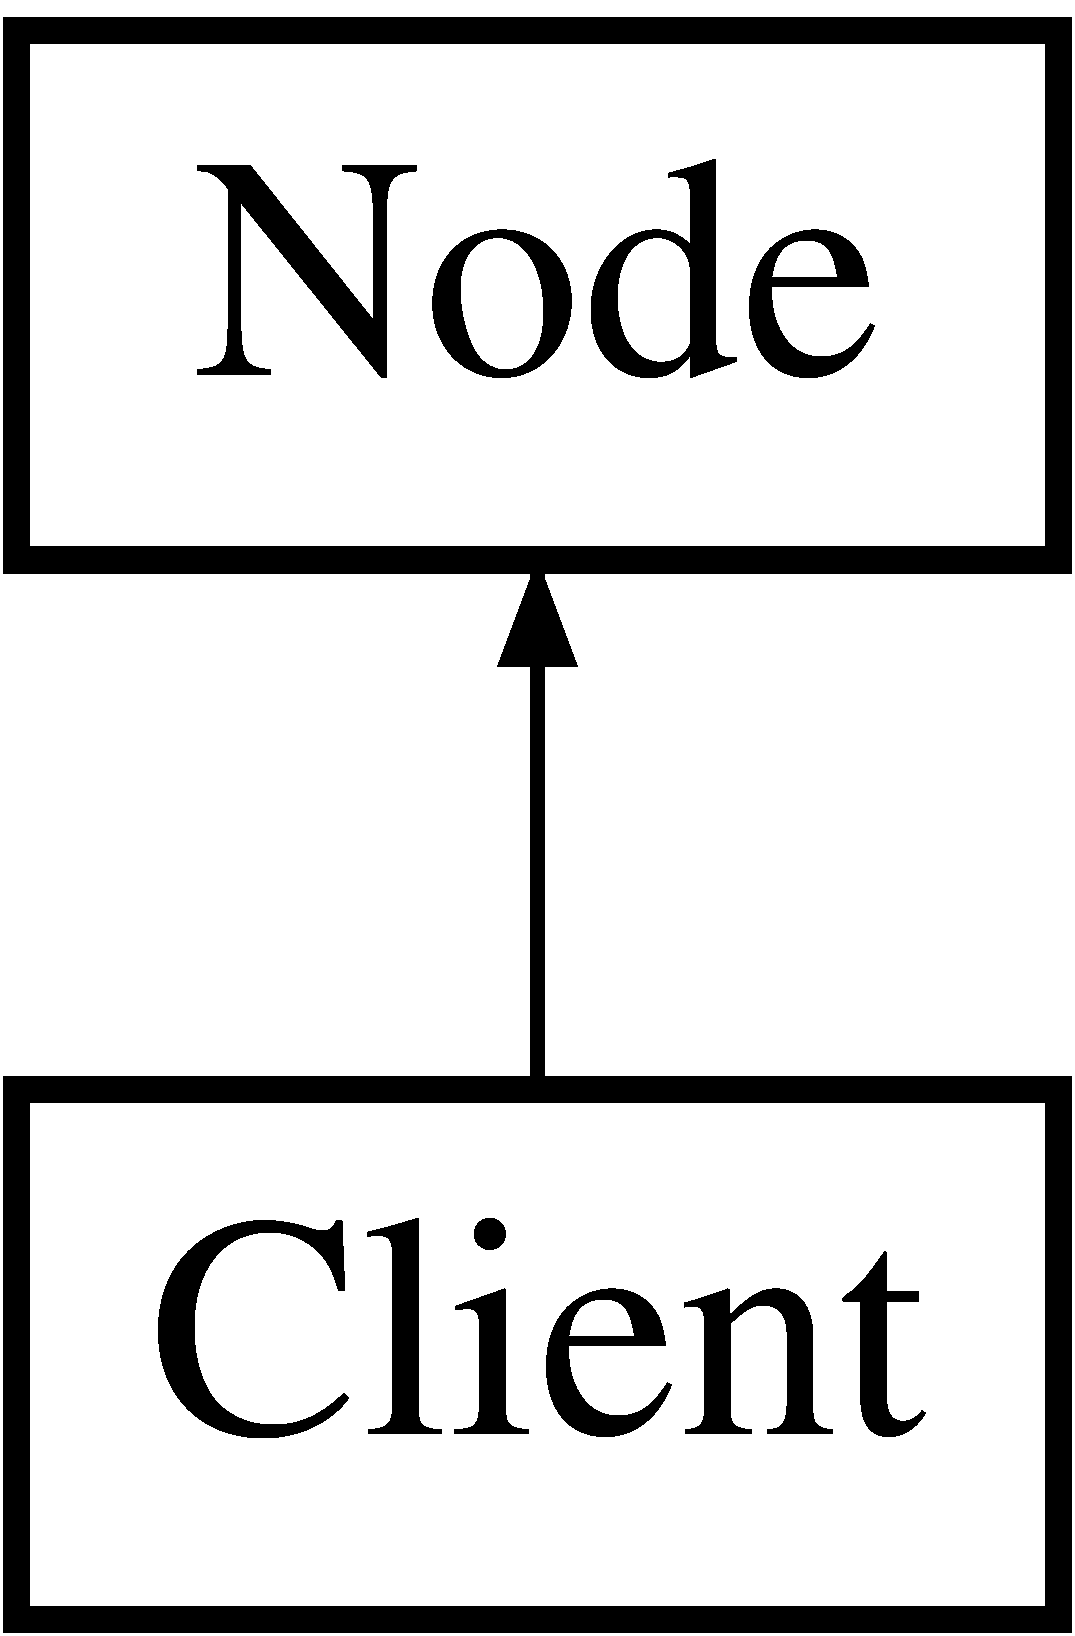
\includegraphics[height=2.000000cm]{classClient}
\end{center}
\end{figure}
\subsection*{Public Member Functions}
\begin{DoxyCompactItemize}
\item 
int \hyperlink{classClient_a5de857af6e3c568925ecd342314617d7}{initialize} ()
\item 
int \hyperlink{classClient_a90a2db07daa07b38544fe3724520f4da}{connect\-\_\-servers} ()
\item 
{\footnotesize template$<$typename K , typename V $>$ }\\int \hyperlink{classClient_aaa4866468879b4e1f6905756191e20d1}{put} (K key, V value)
\item 
{\footnotesize template$<$typename K , typename V $>$ }\\V \hyperlink{classClient_a12d1464831984d5d90358a2abb75f405}{get} (K key)
\item 
{\footnotesize template$<$typename K $>$ }\\\hyperlink{classServer}{Server} $\ast$ \hyperlink{classClient_aab8dfc8e80e752a5f0c1feac7d7ec163}{get\-Primary} (K key)
\end{DoxyCompactItemize}
\subsection*{Additional Inherited Members}


\subsection{Detailed Description}
\hyperlink{classClient}{Client} \hyperlink{classNode}{Node} definition 

\subsection{Member Function Documentation}
\hypertarget{classClient_a90a2db07daa07b38544fe3724520f4da}{\index{Client@{Client}!connect\-\_\-servers@{connect\-\_\-servers}}
\index{connect\-\_\-servers@{connect\-\_\-servers}!Client@{Client}}
\subsubsection[{connect\-\_\-servers}]{\setlength{\rightskip}{0pt plus 5cm}int Client\-::connect\-\_\-servers (
\begin{DoxyParamCaption}
{}
\end{DoxyParamCaption}
)}}\label{classClient_a90a2db07daa07b38544fe3724520f4da}
Connect to servers

\begin{DoxyReturn}{Returns}
status. 0 on success, non-\/zero otherwise. 
\end{DoxyReturn}
\hypertarget{classClient_a12d1464831984d5d90358a2abb75f405}{\index{Client@{Client}!get@{get}}
\index{get@{get}!Client@{Client}}
\subsubsection[{get}]{\setlength{\rightskip}{0pt plus 5cm}template$<$typename K , typename V $>$ V Client\-::get (
\begin{DoxyParamCaption}
\item[{K}]{key}
\end{DoxyParamCaption}
)\hspace{0.3cm}{\ttfamily [inline]}}}\label{classClient_a12d1464831984d5d90358a2abb75f405}
Get value in hash table on servers at key


\begin{DoxyParams}{Parameters}
{\em key} & -\/ key to lookup in table\\
\hline
\end{DoxyParams}
\begin{DoxyReturn}{Returns}
value stored in table 
\end{DoxyReturn}
\hypertarget{classClient_aab8dfc8e80e752a5f0c1feac7d7ec163}{\index{Client@{Client}!get\-Primary@{get\-Primary}}
\index{get\-Primary@{get\-Primary}!Client@{Client}}
\subsubsection[{get\-Primary}]{\setlength{\rightskip}{0pt plus 5cm}template$<$typename K $>$ {\bf Server}$\ast$ Client\-::get\-Primary (
\begin{DoxyParamCaption}
\item[{K}]{key}
\end{DoxyParamCaption}
)\hspace{0.3cm}{\ttfamily [inline]}}}\label{classClient_aab8dfc8e80e752a5f0c1feac7d7ec163}
Get the primary server storing a key


\begin{DoxyParams}{Parameters}
{\em key} & -\/ key whose primary server to search for\\
\hline
\end{DoxyParams}
\begin{DoxyReturn}{Returns}
\hyperlink{classServer}{Server} storing key 
\end{DoxyReturn}
\hypertarget{classClient_a5de857af6e3c568925ecd342314617d7}{\index{Client@{Client}!initialize@{initialize}}
\index{initialize@{initialize}!Client@{Client}}
\subsubsection[{initialize}]{\setlength{\rightskip}{0pt plus 5cm}int Client\-::initialize (
\begin{DoxyParamCaption}
{}
\end{DoxyParamCaption}
)\hspace{0.3cm}{\ttfamily [virtual]}}}\label{classClient_a5de857af6e3c568925ecd342314617d7}
Initialize client

\begin{DoxyReturn}{Returns}
status. 0 on success, non-\/zero otherwise. 
\end{DoxyReturn}


Reimplemented from \hyperlink{classNode_acfbc12d3b7d414fb12811041b04a1809}{Node}.

\hypertarget{classClient_aaa4866468879b4e1f6905756191e20d1}{\index{Client@{Client}!put@{put}}
\index{put@{put}!Client@{Client}}
\subsubsection[{put}]{\setlength{\rightskip}{0pt plus 5cm}template$<$typename K , typename V $>$ int Client\-::put (
\begin{DoxyParamCaption}
\item[{K}]{key, }
\item[{V}]{value}
\end{DoxyParamCaption}
)\hspace{0.3cm}{\ttfamily [inline]}}}\label{classClient_aaa4866468879b4e1f6905756191e20d1}
Store key/value pair in hash table on servers


\begin{DoxyParams}{Parameters}
{\em key} & -\/ key to store value at in table \\
\hline
{\em value} & -\/ data value to store in table at key\\
\hline
\end{DoxyParams}
\begin{DoxyReturn}{Returns}
status. 0 on success, non-\/zero otherwise. 
\end{DoxyReturn}


The documentation for this class was generated from the following file\-:\begin{DoxyCompactItemize}
\item 
/root/cjdambro/grad-\/school/\-C\-S\-E498/gits/fault-\/tolerance/include/\hyperlink{fault__tolerance_8h}{fault\-\_\-tolerance.\-h}\end{DoxyCompactItemize}

\hypertarget{classKVCGConfig}{}\section{K\+V\+C\+G\+Config Class Reference}
\label{classKVCGConfig}\index{K\+V\+C\+G\+Config@{K\+V\+C\+G\+Config}}


{\ttfamily \#include $<$kvcg\+\_\+config.\+h$>$}

\subsection*{Public Member Functions}
\begin{DoxyCompactItemize}
\item 
int \mbox{\hyperlink{classKVCGConfig_a47206f279489aacccb9200f0bf9b36cf}{parse\+\_\+json\+\_\+file}} (std\+::string filename)
\item 
std\+::size\+\_\+t \mbox{\hyperlink{classKVCGConfig_a873ecf819a05b79ccced5e5dada7843f}{get\+\_\+checksum}} ()
\item 
std\+::vector$<$ \mbox{\hyperlink{classft_1_1Server}{ft\+::\+Server}} $\ast$ $>$ \mbox{\hyperlink{classKVCGConfig_a260449f62666e968566716e2ea2c47c2}{get\+Server\+List}} ()
\item 
cse498\+::\+Provider\+Type \mbox{\hyperlink{classKVCGConfig_a66862a874ddbbe54e7b696894b970539}{get\+Provider}} ()
\item 
int \mbox{\hyperlink{classKVCGConfig_a971fafd747cbe1c95f1253d80e5549c6}{get\+Server\+Port}} ()
\item 
int \mbox{\hyperlink{classKVCGConfig_a4c25599c2f79b6ad5acd5e03526864be}{get\+Client\+Port}} ()
\end{DoxyCompactItemize}


\subsection{Detailed Description}
Class to parse config file and store data 

\subsection{Member Function Documentation}
\mbox{\Hypertarget{classKVCGConfig_a873ecf819a05b79ccced5e5dada7843f}\label{classKVCGConfig_a873ecf819a05b79ccced5e5dada7843f}} 
\index{K\+V\+C\+G\+Config@{K\+V\+C\+G\+Config}!get\+\_\+checksum@{get\+\_\+checksum}}
\index{get\+\_\+checksum@{get\+\_\+checksum}!K\+V\+C\+G\+Config@{K\+V\+C\+G\+Config}}
\subsubsection{\texorpdfstring{get\+\_\+checksum()}{get\_checksum()}}
{\footnotesize\ttfamily std\+::size\+\_\+t K\+V\+C\+G\+Config\+::get\+\_\+checksum (\begin{DoxyParamCaption}{ }\end{DoxyParamCaption})}

Calculate and return a checksum for the configuration.

\begin{DoxyReturn}{Returns}
hash of config file 
\end{DoxyReturn}
\mbox{\Hypertarget{classKVCGConfig_a4c25599c2f79b6ad5acd5e03526864be}\label{classKVCGConfig_a4c25599c2f79b6ad5acd5e03526864be}} 
\index{K\+V\+C\+G\+Config@{K\+V\+C\+G\+Config}!get\+Client\+Port@{get\+Client\+Port}}
\index{get\+Client\+Port@{get\+Client\+Port}!K\+V\+C\+G\+Config@{K\+V\+C\+G\+Config}}
\subsubsection{\texorpdfstring{get\+Client\+Port()}{getClientPort()}}
{\footnotesize\ttfamily int K\+V\+C\+G\+Config\+::get\+Client\+Port (\begin{DoxyParamCaption}{ }\end{DoxyParamCaption})\hspace{0.3cm}{\ttfamily [inline]}}

Get the port for server-\/client communication

\begin{DoxyReturn}{Returns}
int for client port 
\end{DoxyReturn}
\mbox{\Hypertarget{classKVCGConfig_a66862a874ddbbe54e7b696894b970539}\label{classKVCGConfig_a66862a874ddbbe54e7b696894b970539}} 
\index{K\+V\+C\+G\+Config@{K\+V\+C\+G\+Config}!get\+Provider@{get\+Provider}}
\index{get\+Provider@{get\+Provider}!K\+V\+C\+G\+Config@{K\+V\+C\+G\+Config}}
\subsubsection{\texorpdfstring{get\+Provider()}{getProvider()}}
{\footnotesize\ttfamily cse498\+::\+Provider\+Type K\+V\+C\+G\+Config\+::get\+Provider (\begin{DoxyParamCaption}{ }\end{DoxyParamCaption})\hspace{0.3cm}{\ttfamily [inline]}}

Get the provider from config.

\begin{DoxyReturn}{Returns}
Provider\+Type for servers. 
\end{DoxyReturn}
\mbox{\Hypertarget{classKVCGConfig_a260449f62666e968566716e2ea2c47c2}\label{classKVCGConfig_a260449f62666e968566716e2ea2c47c2}} 
\index{K\+V\+C\+G\+Config@{K\+V\+C\+G\+Config}!get\+Server\+List@{get\+Server\+List}}
\index{get\+Server\+List@{get\+Server\+List}!K\+V\+C\+G\+Config@{K\+V\+C\+G\+Config}}
\subsubsection{\texorpdfstring{get\+Server\+List()}{getServerList()}}
{\footnotesize\ttfamily std\+::vector$<$\mbox{\hyperlink{classft_1_1Server}{ft\+::\+Server}}$\ast$$>$ K\+V\+C\+G\+Config\+::get\+Server\+List (\begin{DoxyParamCaption}{ }\end{DoxyParamCaption})\hspace{0.3cm}{\ttfamily [inline]}}

Get list of servers parsed from config.

\begin{DoxyReturn}{Returns}
vector of Servers 
\end{DoxyReturn}
\mbox{\Hypertarget{classKVCGConfig_a971fafd747cbe1c95f1253d80e5549c6}\label{classKVCGConfig_a971fafd747cbe1c95f1253d80e5549c6}} 
\index{K\+V\+C\+G\+Config@{K\+V\+C\+G\+Config}!get\+Server\+Port@{get\+Server\+Port}}
\index{get\+Server\+Port@{get\+Server\+Port}!K\+V\+C\+G\+Config@{K\+V\+C\+G\+Config}}
\subsubsection{\texorpdfstring{get\+Server\+Port()}{getServerPort()}}
{\footnotesize\ttfamily int K\+V\+C\+G\+Config\+::get\+Server\+Port (\begin{DoxyParamCaption}{ }\end{DoxyParamCaption})\hspace{0.3cm}{\ttfamily [inline]}}

Get the port for server-\/to-\/server communication

\begin{DoxyReturn}{Returns}
int for server port 
\end{DoxyReturn}
\mbox{\Hypertarget{classKVCGConfig_a47206f279489aacccb9200f0bf9b36cf}\label{classKVCGConfig_a47206f279489aacccb9200f0bf9b36cf}} 
\index{K\+V\+C\+G\+Config@{K\+V\+C\+G\+Config}!parse\+\_\+json\+\_\+file@{parse\+\_\+json\+\_\+file}}
\index{parse\+\_\+json\+\_\+file@{parse\+\_\+json\+\_\+file}!K\+V\+C\+G\+Config@{K\+V\+C\+G\+Config}}
\subsubsection{\texorpdfstring{parse\+\_\+json\+\_\+file()}{parse\_json\_file()}}
{\footnotesize\ttfamily int K\+V\+C\+G\+Config\+::parse\+\_\+json\+\_\+file (\begin{DoxyParamCaption}\item[{std\+::string}]{filename }\end{DoxyParamCaption})}

Parse J\+S\+ON input file


\begin{DoxyParams}{Parameters}
{\em filename} & -\/ name of J\+S\+ON file to parse\\
\hline
\end{DoxyParams}
\begin{DoxyReturn}{Returns}
status. 0 on success, non-\/zero otherwise. 
\end{DoxyReturn}


The documentation for this class was generated from the following file\+:\begin{DoxyCompactItemize}
\item 
/root/cjdambro/grad-\/school/\+C\+S\+E498/gits/fault-\/tolerance/include/faulttolerance/kvcg\+\_\+config.\+h\end{DoxyCompactItemize}

\hypertarget{classNode}{\section{Node Class Reference}
\label{classNode}\index{Node@{Node}}
}
Inheritance diagram for Node\-:\begin{figure}[H]
\begin{center}
\leavevmode
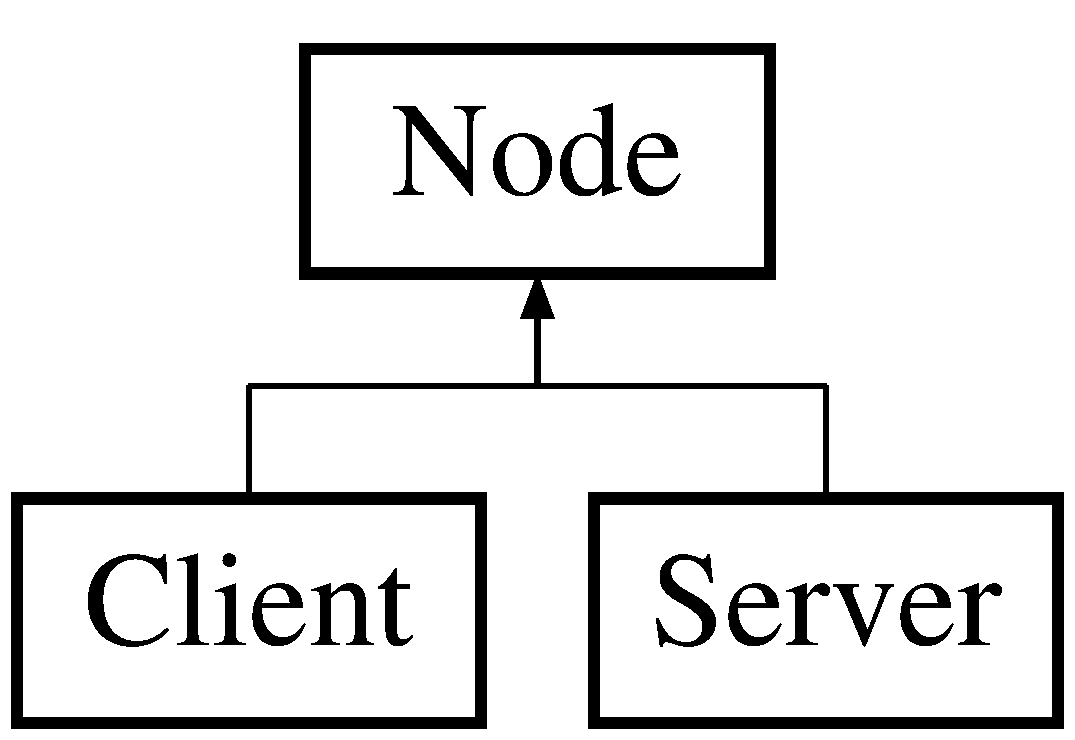
\includegraphics[height=2.000000cm]{classNode}
\end{center}
\end{figure}
\subsection*{Public Member Functions}
\begin{DoxyCompactItemize}
\item 
\hypertarget{classNode_acfbc12d3b7d414fb12811041b04a1809}{virtual int {\bfseries initialize} ()}\label{classNode_acfbc12d3b7d414fb12811041b04a1809}

\item 
\hypertarget{classNode_af79916b6bb2580b7cf9397bdeb172988}{void {\bfseries set\-Name} (std\-::string n)}\label{classNode_af79916b6bb2580b7cf9397bdeb172988}

\item 
\hypertarget{classNode_a3e5ac6b5881a3a9d82f3112953c1e546}{std\-::string {\bfseries get\-Name} ()}\label{classNode_a3e5ac6b5881a3a9d82f3112953c1e546}

\end{DoxyCompactItemize}
\subsection*{Protected Attributes}
\begin{DoxyCompactItemize}
\item 
\hypertarget{classNode_a9f5a57e15567a0b92cb8d25bcec7bd24}{std\-::string {\bfseries hostname}}\label{classNode_a9f5a57e15567a0b92cb8d25bcec7bd24}

\end{DoxyCompactItemize}


The documentation for this class was generated from the following file\-:\begin{DoxyCompactItemize}
\item 
/root/cjdambro/grad-\/school/\-C\-S\-E498/gits/fault-\/tolerance/include/\hyperlink{fault__tolerance_8h}{fault\-\_\-tolerance.\-h}\end{DoxyCompactItemize}

\hypertarget{classServer}{}\doxysection{Server Class Reference}
\label{classServer}\index{Server@{Server}}


{\ttfamily \#include $<$fault\+\_\+tolerance.\+h$>$}

Inheritance diagram for Server\+:\begin{figure}[H]
\begin{center}
\leavevmode
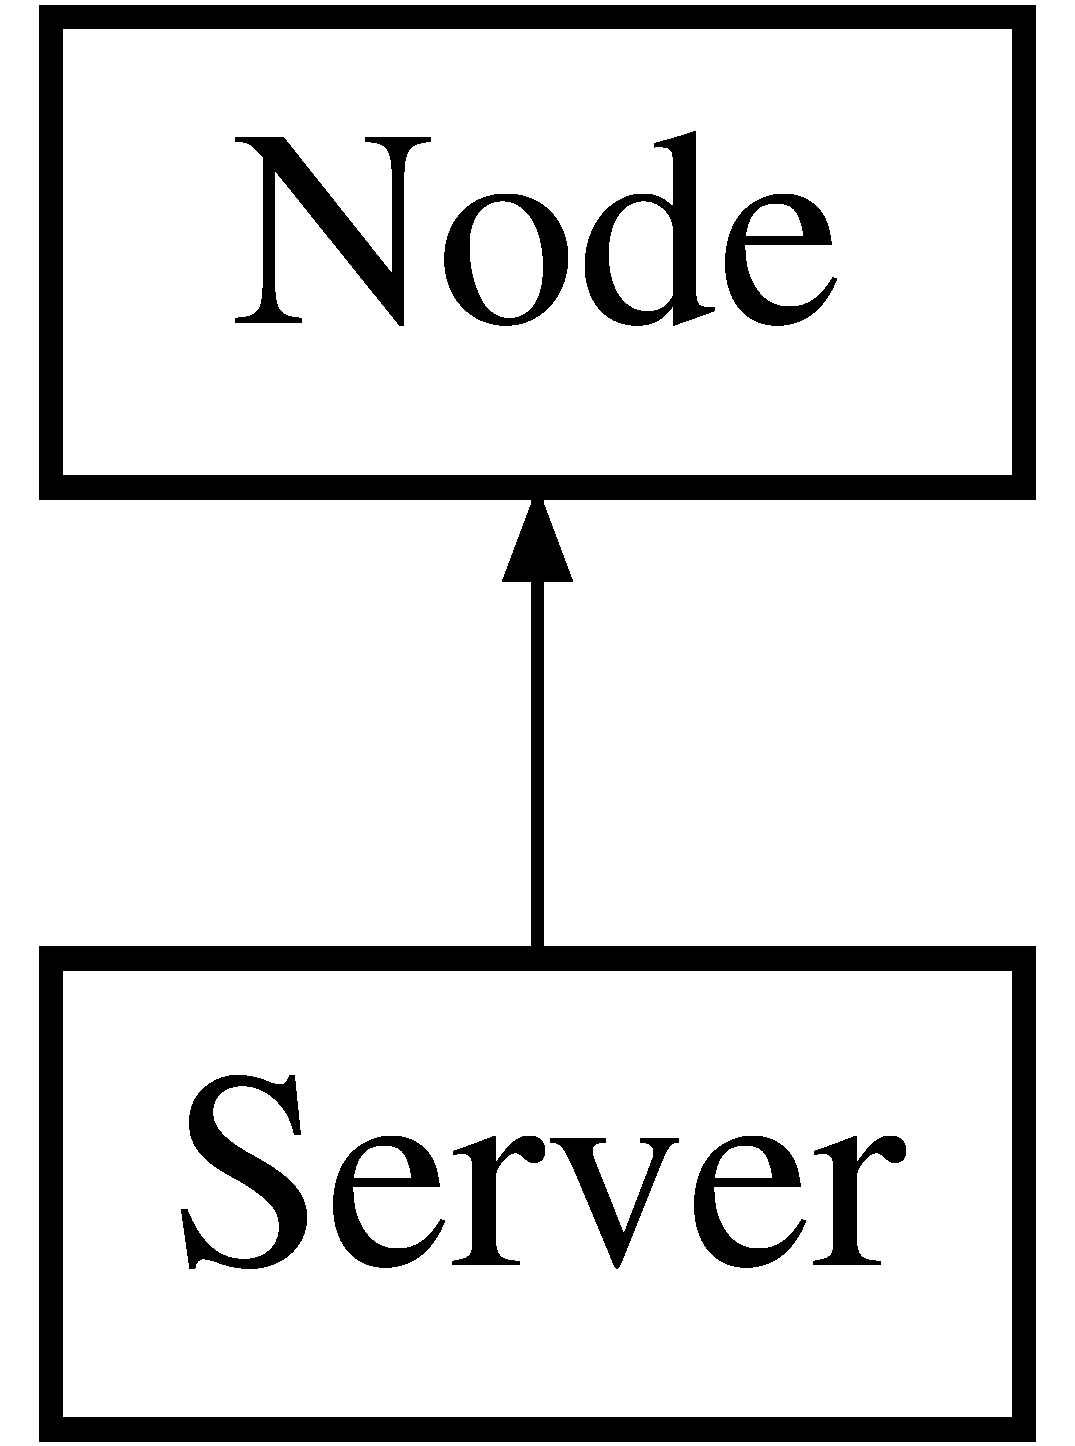
\includegraphics[height=2.000000cm]{classServer}
\end{center}
\end{figure}
\doxysubsection*{Public Member Functions}
\begin{DoxyCompactItemize}
\item 
int \mbox{\hyperlink{classServer_ae94d08657f48a3b51b411463f1137375}{initialize}} ()
\item 
void \mbox{\hyperlink{classServer_a4ce7fd6ac1a1f940db29e57f5f33ae9b}{shutdown\+Server}} ()
\item 
void \mbox{\hyperlink{classServer_aafbaecfe9f27c9eeb811a1bfde5e6c2e}{print\+Server}} (Log\+Level lvl)
\item 
std\+::vector$<$ std\+::pair$<$ int, int $>$ $>$ \mbox{\hyperlink{classServer_ad303d839086eee11137e6fc4a4bb95ab}{get\+Primary\+Keys}} ()
\item 
bool \mbox{\hyperlink{classServer_a395d7cb7194064c961710663926e4a3d}{add\+Key\+Range}} (std\+::pair$<$ int, int $>$ key\+Range)
\item 
bool \mbox{\hyperlink{classServer_a2f865f52beecb3be03eda85b4dc64e3e}{add\+Primary\+Server}} (\mbox{\hyperlink{classServer}{Server}} $\ast$s)
\item 
std\+::vector$<$ \mbox{\hyperlink{classServer}{Server}} $\ast$ $>$ \mbox{\hyperlink{classServer_a71a34c248da1cb74f3453f06223a606e}{get\+Backup\+Servers}} ()
\item 
bool \mbox{\hyperlink{classServer_ab272570a3b1d8eb7f9037c9e7b4e5f2a}{add\+Backup\+Server}} (\mbox{\hyperlink{classServer}{Server}} $\ast$s)
\item 
bool \mbox{\hyperlink{classServer_a9bd7a3b2b12f2f5bddd68eb245111d02}{is\+Primary}} (int key)
\item 
bool \mbox{\hyperlink{classServer_a66708ca0f53116a15258353cc60d1fd4}{is\+Backup}} (int key)
\item 
{\footnotesize template$<$typename K , typename V $>$ }\\int \mbox{\hyperlink{classServer_afb4289a5db1c23ac566dbb085a8f91fb}{log\+\_\+put}} (K key, V value)
\item 
{\footnotesize template$<$typename K , typename V $>$ }\\int \mbox{\hyperlink{classServer_ae419ba1245066b80f42302bb0c86ed00}{log\+\_\+put}} (std\+::vector$<$ K $>$ keys, std\+::vector$<$ V $>$ values)
\item 
std\+::size\+\_\+t \mbox{\hyperlink{classServer_adecf34082977620ca31ca8eab317cf6d}{get\+Hash}} ()
\item 
\mbox{\hyperlink{structnet__data__t}{net\+\_\+data\+\_\+t}} \mbox{\hyperlink{classServer_a6cb0d3961a37e1223b25f83b10844f3e}{get\+Net\+Data}} ()
\item 
void \mbox{\hyperlink{classServer_a369a1c0713310bf367b20e69259ac507}{set\+Socket}} (int socket)
\end{DoxyCompactItemize}
\doxysubsection*{Additional Inherited Members}


\doxysubsection{Detailed Description}
\mbox{\hyperlink{classServer}{Server}} \mbox{\hyperlink{classNode}{Node}} definition 

\doxysubsection{Member Function Documentation}
\mbox{\Hypertarget{classServer_ab272570a3b1d8eb7f9037c9e7b4e5f2a}\label{classServer_ab272570a3b1d8eb7f9037c9e7b4e5f2a}} 
\index{Server@{Server}!addBackupServer@{addBackupServer}}
\index{addBackupServer@{addBackupServer}!Server@{Server}}
\doxysubsubsection{\texorpdfstring{addBackupServer()}{addBackupServer()}}
{\footnotesize\ttfamily bool Server\+::add\+Backup\+Server (\begin{DoxyParamCaption}\item[{\mbox{\hyperlink{classServer}{Server}} $\ast$}]{s }\end{DoxyParamCaption})}

Add server who is backing this one up


\begin{DoxyParams}{Parameters}
{\em s} & -\/ \mbox{\hyperlink{classServer}{Server}} to add to backup server list\\
\hline
\end{DoxyParams}
\begin{DoxyReturn}{Returns}
true if added successfully, false otherwise 
\end{DoxyReturn}
\mbox{\Hypertarget{classServer_a395d7cb7194064c961710663926e4a3d}\label{classServer_a395d7cb7194064c961710663926e4a3d}} 
\index{Server@{Server}!addKeyRange@{addKeyRange}}
\index{addKeyRange@{addKeyRange}!Server@{Server}}
\doxysubsubsection{\texorpdfstring{addKeyRange()}{addKeyRange()}}
{\footnotesize\ttfamily bool Server\+::add\+Key\+Range (\begin{DoxyParamCaption}\item[{std\+::pair$<$ int, int $>$}]{key\+Range }\end{DoxyParamCaption})}

Add key range to primary list


\begin{DoxyParams}{Parameters}
{\em key\+Range} & -\/ pair of min and max key\\
\hline
\end{DoxyParams}
\begin{DoxyReturn}{Returns}
true if added successfully, false otherwise 
\end{DoxyReturn}
\mbox{\Hypertarget{classServer_a2f865f52beecb3be03eda85b4dc64e3e}\label{classServer_a2f865f52beecb3be03eda85b4dc64e3e}} 
\index{Server@{Server}!addPrimaryServer@{addPrimaryServer}}
\index{addPrimaryServer@{addPrimaryServer}!Server@{Server}}
\doxysubsubsection{\texorpdfstring{addPrimaryServer()}{addPrimaryServer()}}
{\footnotesize\ttfamily bool Server\+::add\+Primary\+Server (\begin{DoxyParamCaption}\item[{\mbox{\hyperlink{classServer}{Server}} $\ast$}]{s }\end{DoxyParamCaption})}

Add server who this one is backing up


\begin{DoxyParams}{Parameters}
{\em s} & -\/ \mbox{\hyperlink{classServer}{Server}} to add to primary server list\\
\hline
\end{DoxyParams}
\begin{DoxyReturn}{Returns}
true if added successfully, false otherwise 
\end{DoxyReturn}
\mbox{\Hypertarget{classServer_a71a34c248da1cb74f3453f06223a606e}\label{classServer_a71a34c248da1cb74f3453f06223a606e}} 
\index{Server@{Server}!getBackupServers@{getBackupServers}}
\index{getBackupServers@{getBackupServers}!Server@{Server}}
\doxysubsubsection{\texorpdfstring{getBackupServers()}{getBackupServers()}}
{\footnotesize\ttfamily std\+::vector$<$\mbox{\hyperlink{classServer}{Server}}$\ast$$>$ Server\+::get\+Backup\+Servers (\begin{DoxyParamCaption}{ }\end{DoxyParamCaption})\hspace{0.3cm}{\ttfamily [inline]}}

Get list of servers acting as this one\textquotesingle{}s backup

\begin{DoxyReturn}{Returns}
vector of backup servers 
\end{DoxyReturn}
\mbox{\Hypertarget{classServer_adecf34082977620ca31ca8eab317cf6d}\label{classServer_adecf34082977620ca31ca8eab317cf6d}} 
\index{Server@{Server}!getHash@{getHash}}
\index{getHash@{getHash}!Server@{Server}}
\doxysubsubsection{\texorpdfstring{getHash()}{getHash()}}
{\footnotesize\ttfamily std\+::size\+\_\+t Server\+::get\+Hash (\begin{DoxyParamCaption}{ }\end{DoxyParamCaption})}

Get a hash value of this server configuration

\begin{DoxyReturn}{Returns}
hash of the server 
\end{DoxyReturn}
\mbox{\Hypertarget{classServer_a6cb0d3961a37e1223b25f83b10844f3e}\label{classServer_a6cb0d3961a37e1223b25f83b10844f3e}} 
\index{Server@{Server}!getNetData@{getNetData}}
\index{getNetData@{getNetData}!Server@{Server}}
\doxysubsubsection{\texorpdfstring{getNetData()}{getNetData()}}
{\footnotesize\ttfamily \mbox{\hyperlink{structnet__data__t}{net\+\_\+data\+\_\+t}} Server\+::get\+Net\+Data (\begin{DoxyParamCaption}{ }\end{DoxyParamCaption})\hspace{0.3cm}{\ttfamily [inline]}}

Get net data for this server

\begin{DoxyReturn}{Returns}
\mbox{\hyperlink{structnet__data__t}{net\+\_\+data\+\_\+t}} struct 
\end{DoxyReturn}
\mbox{\Hypertarget{classServer_ad303d839086eee11137e6fc4a4bb95ab}\label{classServer_ad303d839086eee11137e6fc4a4bb95ab}} 
\index{Server@{Server}!getPrimaryKeys@{getPrimaryKeys}}
\index{getPrimaryKeys@{getPrimaryKeys}!Server@{Server}}
\doxysubsubsection{\texorpdfstring{getPrimaryKeys()}{getPrimaryKeys()}}
{\footnotesize\ttfamily std\+::vector$<$std\+::pair$<$int, int$>$ $>$ Server\+::get\+Primary\+Keys (\begin{DoxyParamCaption}{ }\end{DoxyParamCaption})\hspace{0.3cm}{\ttfamily [inline]}}

Get vector of primary key ranges

\begin{DoxyReturn}{Returns}
vector of min/max key range pairs 
\end{DoxyReturn}
\mbox{\Hypertarget{classServer_ae94d08657f48a3b51b411463f1137375}\label{classServer_ae94d08657f48a3b51b411463f1137375}} 
\index{Server@{Server}!initialize@{initialize}}
\index{initialize@{initialize}!Server@{Server}}
\doxysubsubsection{\texorpdfstring{initialize()}{initialize()}}
{\footnotesize\ttfamily int Server\+::initialize (\begin{DoxyParamCaption}{ }\end{DoxyParamCaption})\hspace{0.3cm}{\ttfamily [virtual]}}

Initialize server

\begin{DoxyReturn}{Returns}
status. 0 on success, non-\/zero otherwise. 
\end{DoxyReturn}


Reimplemented from \mbox{\hyperlink{classNode_acfbc12d3b7d414fb12811041b04a1809}{Node}}.

\mbox{\Hypertarget{classServer_a66708ca0f53116a15258353cc60d1fd4}\label{classServer_a66708ca0f53116a15258353cc60d1fd4}} 
\index{Server@{Server}!isBackup@{isBackup}}
\index{isBackup@{isBackup}!Server@{Server}}
\doxysubsubsection{\texorpdfstring{isBackup()}{isBackup()}}
{\footnotesize\ttfamily bool Server\+::is\+Backup (\begin{DoxyParamCaption}\item[{int}]{key }\end{DoxyParamCaption})}

Check if server is backing up a given key


\begin{DoxyParams}{Parameters}
{\em key} & -\/ key to check if backing up\\
\hline
\end{DoxyParams}
\begin{DoxyReturn}{Returns}
true if backing, false otherwise 
\end{DoxyReturn}
\mbox{\Hypertarget{classServer_a9bd7a3b2b12f2f5bddd68eb245111d02}\label{classServer_a9bd7a3b2b12f2f5bddd68eb245111d02}} 
\index{Server@{Server}!isPrimary@{isPrimary}}
\index{isPrimary@{isPrimary}!Server@{Server}}
\doxysubsubsection{\texorpdfstring{isPrimary()}{isPrimary()}}
{\footnotesize\ttfamily bool Server\+::is\+Primary (\begin{DoxyParamCaption}\item[{int}]{key }\end{DoxyParamCaption})}

Check if server is running as primary for a given key


\begin{DoxyParams}{Parameters}
{\em key} & -\/ key to check if primary\\
\hline
\end{DoxyParams}
\begin{DoxyReturn}{Returns}
true if primary, false otherwise 
\end{DoxyReturn}
\mbox{\Hypertarget{classServer_afb4289a5db1c23ac566dbb085a8f91fb}\label{classServer_afb4289a5db1c23ac566dbb085a8f91fb}} 
\index{Server@{Server}!log\_put@{log\_put}}
\index{log\_put@{log\_put}!Server@{Server}}
\doxysubsubsection{\texorpdfstring{log\_put()}{log\_put()}\hspace{0.1cm}{\footnotesize\ttfamily [1/2]}}
{\footnotesize\ttfamily template$<$typename K , typename V $>$ \\
int Server\+::log\+\_\+put (\begin{DoxyParamCaption}\item[{K}]{key,  }\item[{V}]{value }\end{DoxyParamCaption})\hspace{0.3cm}{\ttfamily [inline]}}

Log a P\+UT transaction to all backup servers.


\begin{DoxyParams}{Parameters}
{\em key} & -\/ value of key in table \\
\hline
{\em value} & -\/ data to store in table at key\\
\hline
\end{DoxyParams}
\begin{DoxyReturn}{Returns}
0 on success, non-\/zero on failure 
\end{DoxyReturn}
\mbox{\Hypertarget{classServer_ae419ba1245066b80f42302bb0c86ed00}\label{classServer_ae419ba1245066b80f42302bb0c86ed00}} 
\index{Server@{Server}!log\_put@{log\_put}}
\index{log\_put@{log\_put}!Server@{Server}}
\doxysubsubsection{\texorpdfstring{log\_put()}{log\_put()}\hspace{0.1cm}{\footnotesize\ttfamily [2/2]}}
{\footnotesize\ttfamily template$<$typename K , typename V $>$ \\
int Server\+::log\+\_\+put (\begin{DoxyParamCaption}\item[{std\+::vector$<$ K $>$}]{keys,  }\item[{std\+::vector$<$ V $>$}]{values }\end{DoxyParamCaption})\hspace{0.3cm}{\ttfamily [inline]}}

Log a batch of P\+UT transactions to backup servers.


\begin{DoxyParams}{Parameters}
{\em keys} & -\/ vector of keys to update \\
\hline
{\em values} & -\/ vector of data to store at keys\\
\hline
\end{DoxyParams}
\begin{DoxyReturn}{Returns}
0 on success, non-\/zero on failure 
\end{DoxyReturn}
\mbox{\Hypertarget{classServer_aafbaecfe9f27c9eeb811a1bfde5e6c2e}\label{classServer_aafbaecfe9f27c9eeb811a1bfde5e6c2e}} 
\index{Server@{Server}!printServer@{printServer}}
\index{printServer@{printServer}!Server@{Server}}
\doxysubsubsection{\texorpdfstring{printServer()}{printServer()}}
{\footnotesize\ttfamily void Server\+::print\+Server (\begin{DoxyParamCaption}\item[{Log\+Level}]{lvl }\end{DoxyParamCaption})}

Print server configuration if log level $>$ lvl


\begin{DoxyParams}{Parameters}
{\em lvl} & -\/ log level to start printing. Will print more at higher levels. \\
\hline
\end{DoxyParams}
\mbox{\Hypertarget{classServer_a369a1c0713310bf367b20e69259ac507}\label{classServer_a369a1c0713310bf367b20e69259ac507}} 
\index{Server@{Server}!setSocket@{setSocket}}
\index{setSocket@{setSocket}!Server@{Server}}
\doxysubsubsection{\texorpdfstring{setSocket()}{setSocket()}}
{\footnotesize\ttfamily void Server\+::set\+Socket (\begin{DoxyParamCaption}\item[{int}]{socket }\end{DoxyParamCaption})\hspace{0.3cm}{\ttfamily [inline]}}

Set the socket fd for this servers net data


\begin{DoxyParams}{Parameters}
{\em socket} & -\/ socket fd to store \\
\hline
\end{DoxyParams}
\mbox{\Hypertarget{classServer_a4ce7fd6ac1a1f940db29e57f5f33ae9b}\label{classServer_a4ce7fd6ac1a1f940db29e57f5f33ae9b}} 
\index{Server@{Server}!shutdownServer@{shutdownServer}}
\index{shutdownServer@{shutdownServer}!Server@{Server}}
\doxysubsubsection{\texorpdfstring{shutdownServer()}{shutdownServer()}}
{\footnotesize\ttfamily void Server\+::shutdown\+Server (\begin{DoxyParamCaption}{ }\end{DoxyParamCaption})}

Shutdown server 

The documentation for this class was generated from the following file\+:\begin{DoxyCompactItemize}
\item 
/home/runner/work/fault-\/tolerance/fault-\/tolerance/include/\mbox{\hyperlink{fault__tolerance_8h}{fault\+\_\+tolerance.\+h}}\end{DoxyCompactItemize}

\hypertarget{classShard}{}\section{Shard Class Reference}
\label{classShard}\index{Shard@{Shard}}
\subsection*{Public Member Functions}
\begin{DoxyCompactItemize}
\item 
\mbox{\Hypertarget{classShard_a022ca4cc62df25d9311672c7bec01695}\label{classShard_a022ca4cc62df25d9311672c7bec01695}} 
{\bfseries Shard} (std\+::pair$<$ uint64\+\_\+t, uint64\+\_\+t $>$ kr)
\item 
\mbox{\Hypertarget{classShard_ae55ed3a96bf34e767e3bc836371d6a05}\label{classShard_ae55ed3a96bf34e767e3bc836371d6a05}} 
void {\bfseries add\+Server} (\mbox{\hyperlink{classServer}{Server}} $\ast$s)
\item 
\mbox{\Hypertarget{classShard_a5caa880343d70450edaa632cdc6b2e36}\label{classShard_a5caa880343d70450edaa632cdc6b2e36}} 
\mbox{\hyperlink{classServer}{Server}} $\ast$ {\bfseries get\+Primary} (bool force)
\item 
\mbox{\Hypertarget{classShard_a6cf4ee2175ea08b1689b3cd917d39e35}\label{classShard_a6cf4ee2175ea08b1689b3cd917d39e35}} 
void {\bfseries set\+Primary} (\mbox{\hyperlink{classServer}{Server}} $\ast$s)
\end{DoxyCompactItemize}


The documentation for this class was generated from the following file\+:\begin{DoxyCompactItemize}
\item 
/root/cjdambro/grad-\/school/\+C\+S\+E498/gits/fault-\/tolerance/include/faulttolerance/shard.\+h\end{DoxyCompactItemize}

\chapter{File Documentation}
\hypertarget{fault__tolerance_8h}{}\section{/root/cjdambro/grad-\/school/\+C\+S\+E498/gits/fault-\/tolerance/include/faulttolerance/fault\+\_\+tolerance.h File Reference}
\label{fault__tolerance_8h}\index{/root/cjdambro/grad-\/school/\+C\+S\+E498/gits/fault-\/tolerance/include/faulttolerance/fault\+\_\+tolerance.\+h@{/root/cjdambro/grad-\/school/\+C\+S\+E498/gits/fault-\/tolerance/include/faulttolerance/fault\+\_\+tolerance.\+h}}


Public A\+PI for K\+V\+CG Fault Tolerance protocol.  


{\ttfamily \#include $<$faulttolerance/node.\+h$>$}\newline
{\ttfamily \#include $<$faulttolerance/server.\+h$>$}\newline
{\ttfamily \#include $<$faulttolerance/client.\+h$>$}\newline


\subsection{Detailed Description}
Public A\+PI for K\+V\+CG Fault Tolerance protocol. 


%--- End generated contents ---

% Index
\backmatter
\newpage
\phantomsection
\clearemptydoublepage
\addcontentsline{toc}{chapter}{Index}
\printindex

\end{document}
